%
% main.tex -- Paper zum Thema wwt
%
% (c) 2019 Michael Schmid, Hochschule Rapperswil
%
\chapter{Wetter-Wavelet-Transformation\label{chapter:wwt}}
\lhead{Wetter-Wavelet-Transformation}
\begin{refsection}
\chapterauthor{Michael Schmid}



\definecolor{codegreen}{rgb}{0,0.6,0}
\definecolor{codegray}{rgb}{0.5,0.5,0.5}
\definecolor{codepurple}{rgb}{0.58,0,0.82}
\definecolor{backcolour}{rgb}{0.95,0.95,0.92}

\lstdefinestyle{mystyle}{
	backgroundcolor=\color{backcolour},   
	commentstyle=\color{codegreen},
	keywordstyle=\color{magenta},
	numberstyle=\tiny\color{codegray},
	stringstyle=\color{codepurple},
	basicstyle=\footnotesize,
	breakatwhitespace=false,         
	breaklines=true,                 
	captionpos=b,                    
	keepspaces=true,                 
	numbers=left,                    
	numbersep=2pt,                  
	showspaces=false,                
	showstringspaces=false,
	showtabs=false,                  
	tabsize=2
}
\lstset{style=mystyle}
\lstdefinestyle{mystyle}{
	morekeywords={cwt,contourf,datetick}
}


\section{Einführung}
\rhead{Einführung}


Seit langen konsultiere ich meine aktuellen Wetterdaten von einer eher unüblichen Internetseite.
Dabei handelt es sich um eine privat geführte Wetterstation, welche die gemessenen Daten kostenlos und sehr rudimentär im Internet grafisch darstellt.
Weiter werden die Daten auch tabellarisch zur Verfügung gestellt.
Das Feature, welches is bis anhin am regelmässigsten nutze, war die grafische Darstellung der aktuellen Wetterdaten über den Zeitraum der letzten 24 Stunden.
Bei speziellen Ereignissen des Wetters, vielen mir besondere und wiederkehrende Charakteristiken auf.
\\
\\
Nach der Einführung in die Theorie der Wavelets kam mir die Idee, solche Wetterphänomene mittels einer geeigneten Wavelet Transformation zu detektieren.
In diesem Paper wird einerseits auf die theoretischen Grundlagen der angewandten Methoden zurückgegriffen sowie die besprochenen meteorologischen Phänomene kurz erläutert. 
Weiterführend wird auf den eigentlichen Prozess des Papers vertieft eingegangen.
Ein besonderes Augenmerk wird auf die allgemeine Vorgehensweise sowie deren Schwierigkeiten gelegt.
\\




\section{Wetterstation Seegräben}
\rhead{Wetterstation Seegräben}

Die  angesprochene Wetterstation ist eine privat geführte Wetterstation in der Gemeinde Seegräben im Kanton Zürich.

Die Wetterstation ist aus einer DAVIS Vantage Pro2 6153 aufgebaut.
Diese besteht aus einem Thermo- und  Hyrosensor, einem Windgeschwindigkeit und Richtungsmesser sowie einem Regenmesser. 
Durch diese Sensoren werden folgende Daten aufgezeichnet:
\\
\\
\\


\begin{itemize}
	\item \textbf{Aussentemperatur} in Grad Celcius
	\item \textbf{Relative Luftfeuchtigkei} in Prozent
	\item \textbf{Luftdruck} in hPa
	\item \textbf{Windgeschwindigkeit} in km/h, gemittelt über 5 Minuten
	\item \textbf{Windböen} in km/h
	\item \textbf{Windrichtung} nach Himmelsrichtung
	\item \textbf{Regenmenge} in l/mm²
\end{itemize}	


Der Thermo- / Hydrosensor liegt zusammen mit dem Regenmengenmesser auf 2 Meter über dem Boden.
Mit einem Abstand von rund 10 Meter zum nächsten Gebäude, werden optimale Messbedingungen geschaffen.
Der Windmesser wurde am First des Gebäudes montiert.
Mit einem Masten werden die Daten 1,5 Meter über dem First gemessen\cite{online:wss}.
Die Daten werden anschliessend mit einer Software von PC-Wetterstation.de weiterverarbeitet und auf eine rudiment\"aren Website dargestellt.
Mehr zur Verwendung der Wetterdaten im n\"achsten Kapitel.

\section{Datenaufarbeitung}
\rhead{Datenaufarbeitung}
Als n\"achster Schritt der Vorbereitung zur Wavelet Transformation, war die Aufbereitung der zur Verf\"ugung gestellten Daten der Wetterstation Seegr\"aben. Dazu musste erst analysiert werden wie die Daten auf der Website dargestellt werden.
\subsection{Wetter-Archiv}
Auf der Website gibt es mehrere Möglichkeiten sich Wetterdaten aus der Vergangenheit darstellen zulassen.
In der Sektion des Archivs kann man die Wetterdaten eines gew\"unschten Zeitraums tabellarisch oder grafisch darstellen lassen.
Von den Betreiber der Website steht keine Funktion zur Verfügung, welche einem erlaubt die Daten offiziell Herunter zu laden.
\subsection{Datenerfassung}
Da f\"ur meine Anwendung eine m\"oglichst genaue Aufl\"osung der jeweiligen Daten erforderlich ist, mussten die Daten im Zeitraum von einem Tag dargestellt werden.
Dies hatte zur Folge, dass man f\"ur jeden Tag ein Tabelle auf dem Archiv der Website \"offnen musste. Man hätte anschliessend die Daten mittel "Copy und Paste" Verfahren in eine Excel-Tabelle einzuf\"ugen können. Es wurde allerdings entschieden, ein Programm zu schreiben welches diese Aufgabe automatisieren sollte.
Als Programmiersprache wurde hierf\"ur Python gewählt.


Mit der Pandas Library und der Funktion "read\_html"\space konnten die Daten direkt mittels Aufruf aus dem Python Programm von der URL-Seite heruntergeladen werden.
Entscheidend für das Gelingen dieser Teilaufgabe war, dass die URL-Links der einzelnen Tage jeweils regelmässig aufgebaut sind.
Da dies der Fall war, konnten die entsprechenden Link mittels einer einfachen While-Schleife zusammengesetzt werden.

Siehe in der Abblindung \ref{fig:python-code} der wesentliche Ausschnitt aus dem Python Code:
\begin{figure}
	\centering
	\lstinputlisting[language=Python,firstline=1,lastline=16,numbers=left,style = mystyle]{papers/wwt/code/get_data.py}
	\caption{Python Codeausschnitt}
	\label{fig:python-code}
\end{figure}

Die Daten konnten im nächsten Schritt in einer Excel-Tabelle abgespeichert werden.
Dort folgte der letzte Feinschliff, dabei wurden alle überflüssigen Kopfzeilen und Statistiken entfernt.

\subsubsection{Unregelmässigkeiten der Wetterstation}
Bei der Datenerfassung durch das eben beschriebene Python Programm wurden einige Unregelmässigkeiten er Wetterstation Seegräben beobachtet.
Das Programm wird jeweils durch einen Fehler abgebrochen, wenn der angegebene Link nicht abrufbar ist. 
So fiel mir auf, dass unregelmässig auf das Jahr verteilt, gewisse Daten von Tagen fehlen. Es stellte sich heraus, dass jeweils die entsprechende Verlinkung zu diesem Datum nicht zur Verfügung steht.
Wenn man manuell auf der Website nach diesem Tag sucht, wird man auch nicht fündig.
Dies trat teilweise sogar in Abschnitten von mehreren Tagen auf.
Wie sich später herausstellte traten die fehlenden Tagen nicht zu den Zeitpunkten auf welche mich interessierten.


\subsection{Datendarstellung}
Die Darstellung der gewonnen Daten konnten einfach mittels Matlab gemacht werden.
Anbei in Abbildung \ref{fig:rawdata} \space die Plot der Rohdaten aus dem Jahre 2018, wobei nur jeder 10 Messpunkt verwendet wurde.
Diese Rohdaten dienten als Grundlage für alle weiteren Berechnungen. 
\begin{figure}
	\centering
	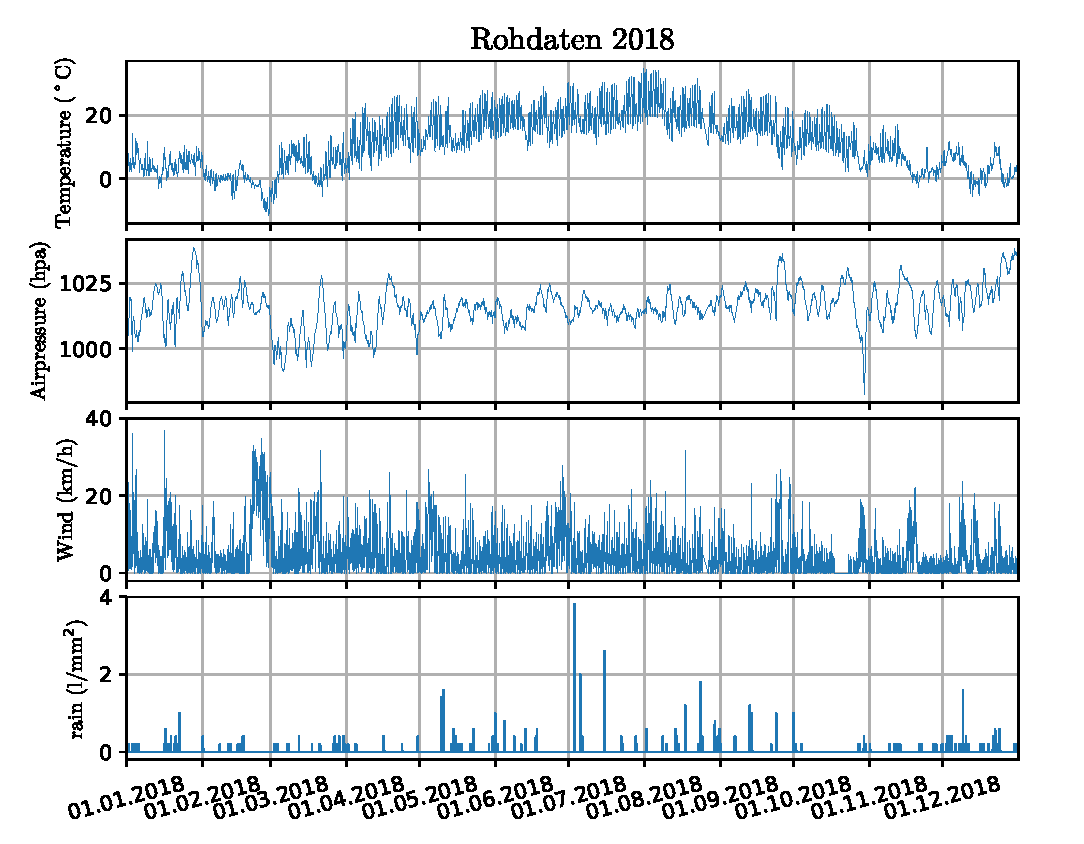
\includegraphics[width=1\textwidth]{papers/wwt/images/raw.pdf}
	\caption{Rohdaten 2018}
	\label{fig:rawdata}
\end{figure}

\newpage
\section{Stetige Wavelet-Transformation}
\rhead{Stetige Wavelet-Transformation}
Die theoretischen Grundlagen rund um die stetige Wavelet-Transformation wurde im Kapitel \ref{chapter:cwt} genaustens erläutert. 
In diesem Abschnitt der Seminararbeit wird öfters auf die Theorie des angesprochene Kapitel \ref{chapter:cwt} referenziert ohne diese weiter zu erläutern. 

Für eine m"oglichst genaue Untersuchung der Signalen, in welcher so viele Information gewonnen werden sollten wie m"oglich, eignet sich die Stetige Wavelet-Transformation (folgend noch kurz \textit{cwt} aus dem Englischen "continuous wavelet transform")
ideal. 
Regelmässig auftretende Frequenzen können dank der \textit{cwt} gefunden und zusätzlich auch einem Zeitraum zugeteilt werden.
\subsection{Verwendetes Wavelet}
In
\begin{equation}
\mathcal{W}f (a,b)
=
\langle f,\psi_{a,b}\rangle
=
\frac{1}{\sqrt{|a|}}\int_{-\infty}^\infty f(t)\,\overline{
	\psi\biggl(\frac{t-b}{a}\biggr)}\,dt
\label{eq:cwt}
\end{equation}
sieht man die Grundlegende Formel der \textit{cwt}.
Wobei das $\psi_{a,b}$ für das Mutter-Wavelet steht, welches mit dem Koeffizienten $a$ skaliert und mit $b$ verschoben wird.

Als Mutter-Wavelet wurde das analytische Gabor-Wavelet verwendet, welches in der Abbildung \ref{fig:gabor_plot} \space dargestellt wird.
\begin{figure}
\centering
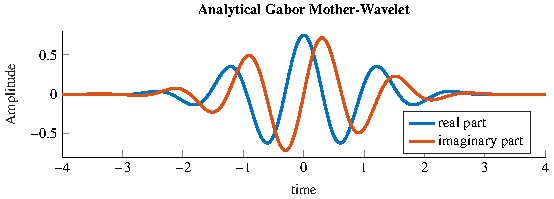
\includegraphics[width=1\textwidth]{papers/wwt/images/gabor.pdf}
\caption{Analytisches Gabor Mutter-Wavelet}
\label{fig:gabor_plot}
\end{figure}

\subsection{Berechung mit Matlab}
Die Berechnung der \textit{cwt} wurde mit der numerischen Berechnugs-Software Matlab durchgeführt.
Die essenzielle Funktion dabei war die cwt()-Funktion.
Die Funktion arbeitete bei korrekter Parametrisierung auch wie gewünscht.
Falls man jedoch genauer verstehen möchte wie die Funktion genau rechnet, muss man sich mit einer eher dürftigen Dokumentation herumschlagen.
Glücklicherweise funktionierte die Funktion für meine Anwendung einwandfrei.
Folgende Parameter wurden verwendet
\lstinputlisting[language=Matlab,firstline=1,lastline=1,  numbers=left, style = mystyle]{papers/wwt/code/matlab.m}
\label{fig:matlab_code_cwt}
wobei Matlab das Gabor-Wavelet als 'amor' bezeichnet, mit 'VoicesPerOctave' konnte die Genauigkeit erhöht werden und die Variabel 'fs' beschreibt die Abtastfrequenz der Messsignale.
Bei den Rückgabewerte werden die Wavelet-Werten in 'wt' als komplexe Matrix und die approximierten Frequenzen in 'F' abgespeichert.

Anstatt den Skalierungsfaktor $a$ in der Gleichung \ref{eq:cwt}, wird eine approximierte Frequenz berechnet und zurückgegeben.
Für jeden verwendeten Skalierungsfaktor $a$ wird eine Sinuskurve gesucht, welche am ehesten der Frequenz des entsprechenden Wavelet übereinstimmt.
Siehe in der Abbindung \ref{fig:centerf} ein Beispiel mit einem Daubechies Wavelet der Nummer 7.
\begin{figure}
	\centering
	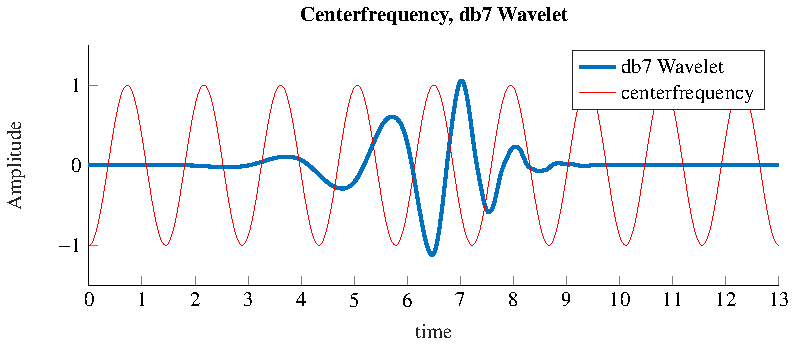
\includegraphics[width=1\textwidth, height=2in]{papers/wwt/images/centerf.pdf}
	\caption{Approximierte Frequenz eines db7-Wavelet}
	\label{fig:centerf}
\end{figure}


\newpage
\subsection{Verifikation approximierte Frequenz}
Diese approximierte Frequenz konnte man mit den geeigneten Daten aus der aktuellen Anwendung der Wetterdaten sehr gut verifizieren.
Der Temperaturverlauf während einer Hochdruckphase ist sehr regelmässig und man sollte den 24 Stunden Tagesverlauf exakt erkennen.

Dank der Regelm"assigkeit des Temperaturverlaufs, sieht man im \textit{cwt}-Plot eine signifikante erh"ohung des Wertes bei einer gewissen Frequenz.
Die Ausgelesene Frequenz beträgt $f = 1.16\cdot10^{-5} \,\text{Hz}$, welches umgerechnet einer Periodendauer von $T = 86206.897\,\text{s}\approx 23\,\text{h }56\,\text{min } 47\,\text{s}$ entspricht.
Damit kann die Frequenz im Rückgabewert der Matlab-Funktion als sehr genau betrachtet werden.
Dabei darf nicht vergessen werden, dass nur alle 5 Minuten einen Datenpunkt aufgenommen wurde, und somit die Abweichung zu 24 Stunden kleiner ist als die Auflösung.
Weiter kommt hinzu, dass jeder Tag zu der Jahreszeit im Frühling ca. 2 Minuten kürzer ist als der jeweils Vorgehende\cite{online:sunset_time}.

\begin{figure}[h]
	\centering
	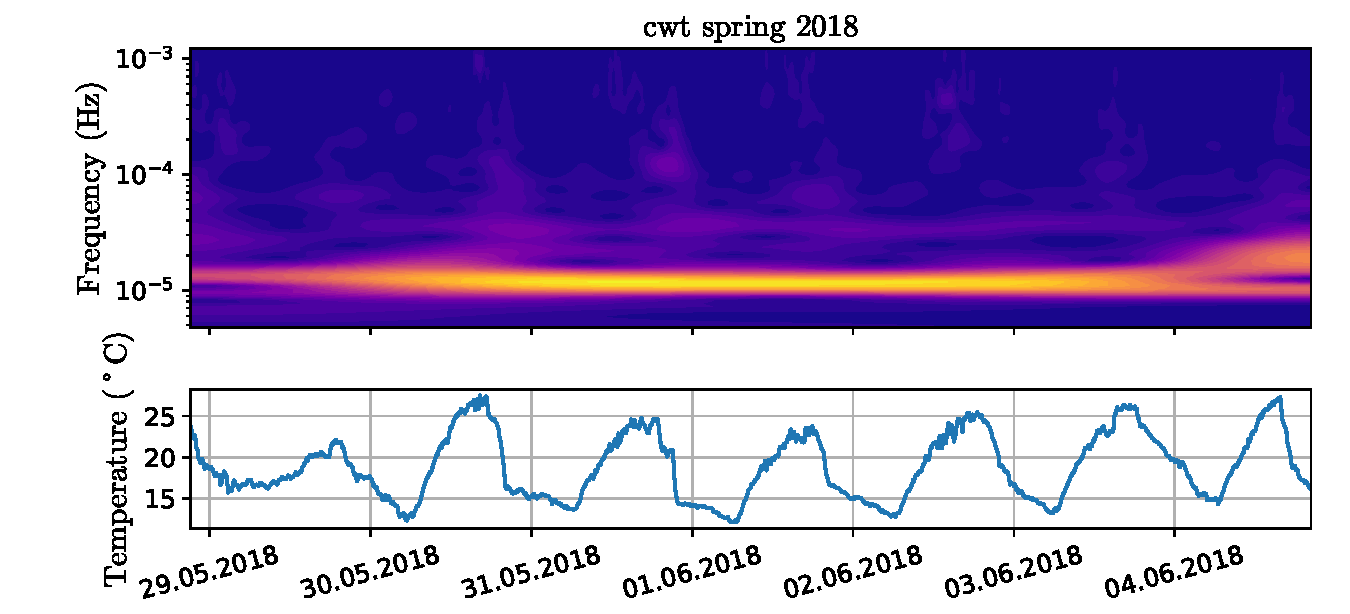
\includegraphics[width=1\textwidth]{papers/wwt/images/data_spring.pdf}
	\caption{Temperaturverlauf und entsp. cwt}
	\label{fig:cwt_zoom}
\end{figure}




\section{Analyse von Wettereignissen}
\rhead{Analyse von Wetterereignissen}
Aufgrund der Kenntnissen rund um die \textit{cwt} wurde die Annahme getroffen, dass signifikante Frequenzereignisse gut detektiert werden können.
Bei einer typischen Sturmfront, welche öfters als Wintersturm in den Monaten Dezember und Januar auftreten, zeigten sich bei der Konsultation der Wetterdaten, rapide Temperatur- und Luftdruckwechsel, sowie ein erhöhtes Windaufkommen.
Das Ziel der Analyse war, solche Ereignisse mittels einer geeigneten \textit{cwr} zu detektieren.
Bei Frontdruchgängen erkennt man rapide Wechsel im Wind, der Temperatur sowie dem Luftdruck.
Diese Gemeinsamkeiten sollte ausgenutzt werden. Diese gemeinsam auftretenden Frequenzen sollten in der \textit{cwt} sichtbar sein.
Um dies zu Verdeutlichen wurden jeweils zwei Messresultate miteinander multipliziert.
Dies funktionierte besonders gut, da die Werte rasch gegen null divergieren falls keine Frequenzen mit dem Mutterwavelet übereinstimmen. 

\subsection{Sturmsaison 2018}
\rhead{Sturmsaison 2018}
Bereits bekannt war, dass in der Sturmsaison im Jahre 2018 einige Winterstürme aufgetreten sind.
So wurde bei der Analyse nur auf diese Periode das Augenmerk gelegt. In Abbildung \ref{fig:cwt_storm} \space sieht man die Wavelet-Transfomrmation des Luftdruckes und Windes miteinander multipliziert. Dies über die Monate Januar und Februar 2018. Auch sieht man den Luftdruck- und Windverlauf.
 
\begin{figure}[h]
	\centering
	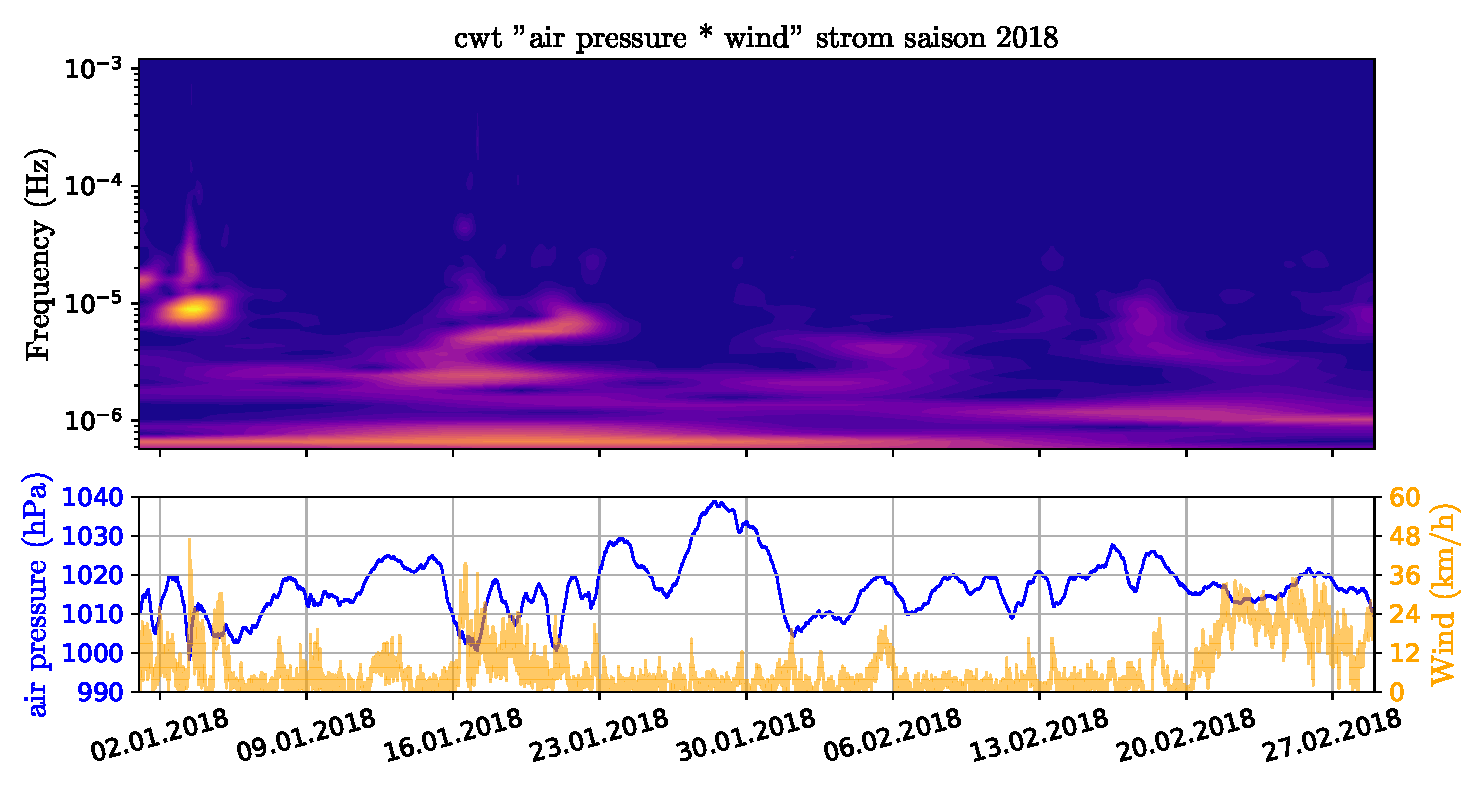
\includegraphics[width=1\textwidth]{papers/wwt/images/storm_airp_wind.pdf}
	\caption{cwt und Rohdaten Sturmsaison 2018}
	\label{fig:cwt_storm}
\end{figure}

in \ref{fig:cwt_storm} \space sieht man um den 3. sowie zwischen dem 16. und 23. Januar jeweils gewisse Frequenzen des Windes und dem Luftdruck welche gemeinsam auf die Wavelet-Transformation angesprochen haben.

\subsubsection{Wintersturm Burglind}
Hineingezoomt in dieses Zeitintervall (Abbildung \ref{fig:cwt_storm_zoom}) sieht man im Rohdatenverlauf die Aktivitäten des Windes und Luftdruckes. 
\begin{figure}[h]
	\centering
	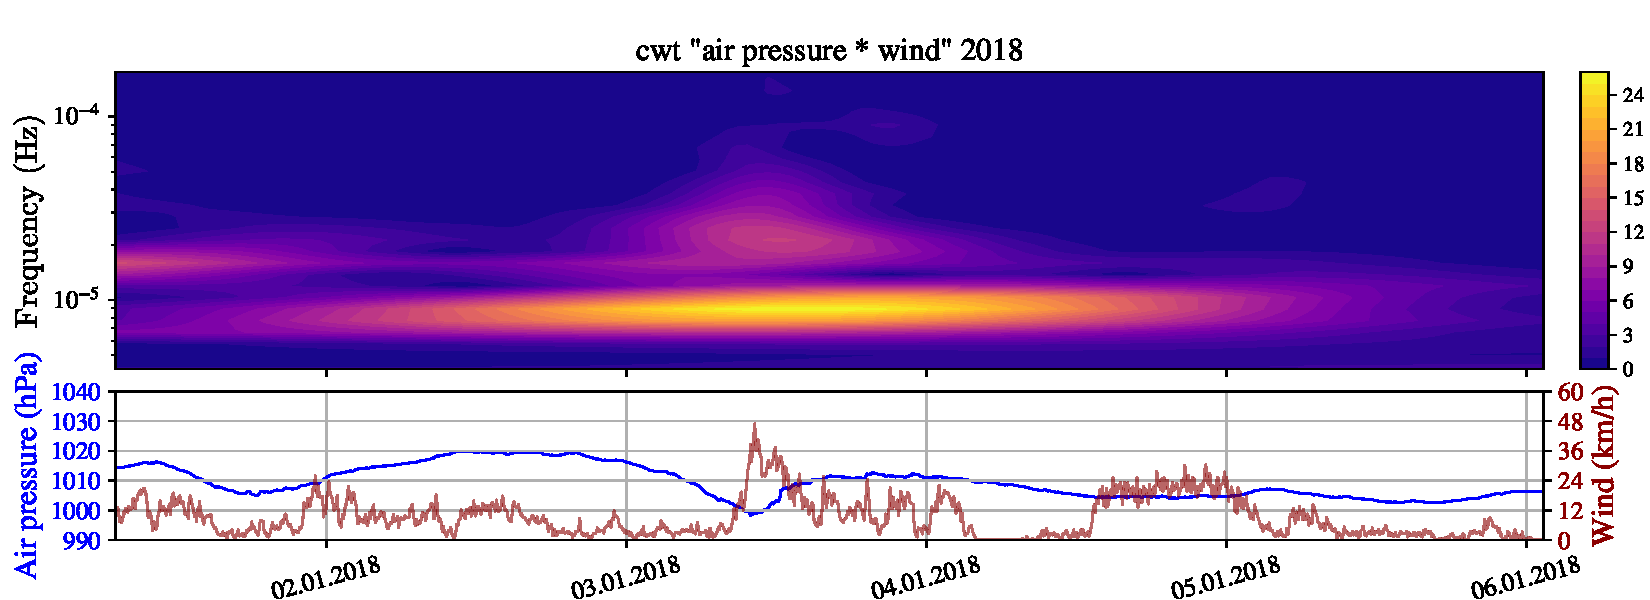
\includegraphics[width=1\textwidth]{papers/wwt/images/storm_airp_wind_zoom.pdf}
	\caption{cwt und Rohdaten Strum 2018}
	\label{fig:cwt_storm_zoom}
\end{figure}
Aus einem Fachbericht von Meteoschweiz war bekannt, dass am Vormittag des 3. Januars 2018 die stärkste Sturmfront seit dem verehrenden Lothar aus dem Jahre 1999 über die Schweiz zog \cite{Fachbericht:Burglind}.
Dabei zeigt sich eindrücklich wie der Sturmdurchgang in der multiplizierten Wavelet-Transformation hervorgehoben wird.

\subsubsection{Sturmtief Evi und Friedericke }
Beim zweiten Ereignis zwischen dem 16. und 23. Januar, trat die Aktivität nicht mehr so deutlich auf.
Nach dem Sturmarchiv\cite{online:sturmarchiv} traf am 16. Januar das Sturmtief Evi und am 18. Januar das Sturmtief Friedericke auf Europa. Dabei zeigt sich nach der Amplitude, dass das Sturmtief nicht direkt auf die Schweiz traf, sonder nur streifte. 

\begin{figure}[h]
	\centering
	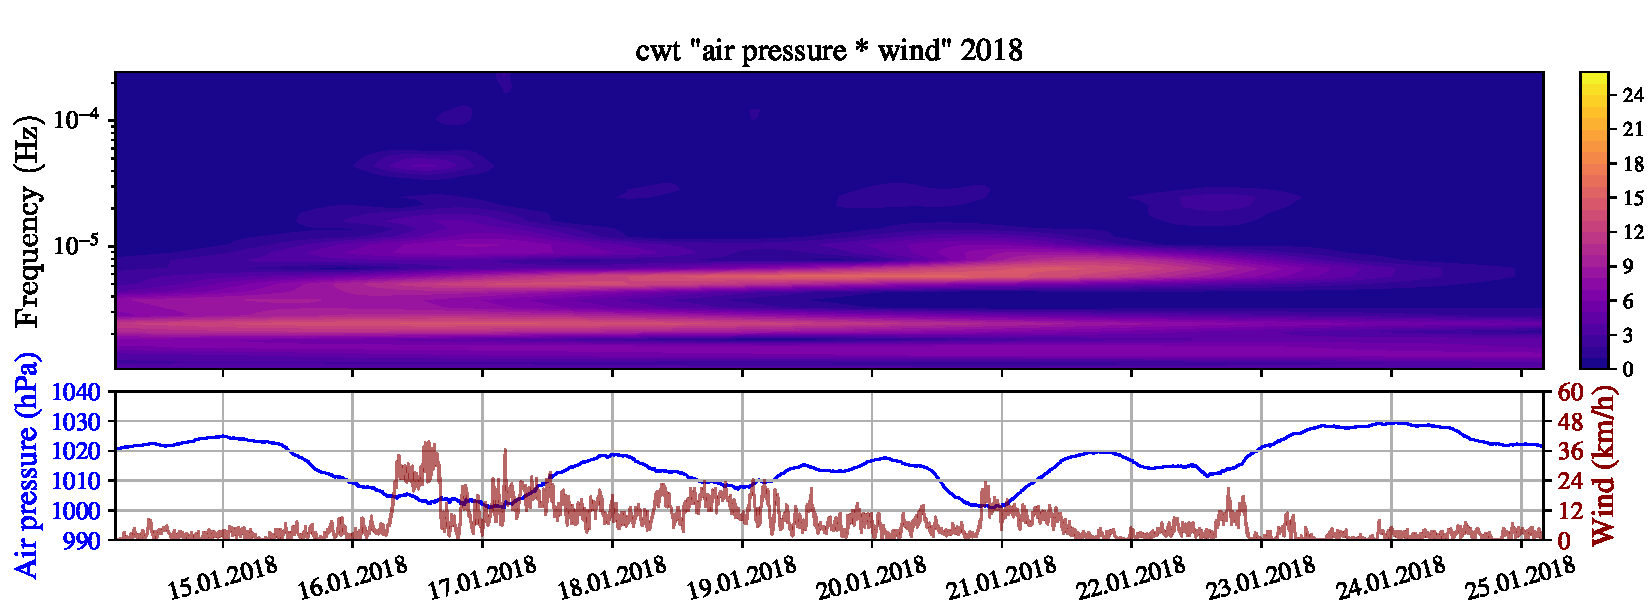
\includegraphics[width=1\textwidth]{papers/wwt/images/storm_airp_wind_zoom2.pdf}
	\caption{cwt und Rohdaten Strum 2018}
	\label{fig:cwt_storm_zoom}
\end{figure}



\section{Schlussfolgerung}
\rhead{Schlussfolgerung}

In diesem Versuch die Wavelet-Transformation im Bereich der Wetteranalyse nützlich zu machen, hat sich gezeigt, dass dies durchaus möglich ist.
In der Anwendung der Winterstürme wurde die Wavelet-Transfomration oder genauer die stetige Wavelet-Transformation erfolgreich eingesetzt.
Die Untersuchten Ereignisse konnten detektiert werden.
Dabei ist selbstverständlich noch nichts abschliessend Bewiesen doch es ist ein Anfang.
Weiterführend müssten mehrere Ereignisse Untersucht werden, um die Analysemethode zu verifizieren.
Auch sollte die Methode weiterführend auf andere metreologische Ereignisse angewandt werden. Zum Beispiel könnte man versuchen Gewitter zu lokalisieren. Falls sich die Methode für mehrere Phänomene beweist, wären die Möglichkeiten zur Anwendung fast Grenzenlos. 
 

\printbibliography[heading=subbibliography]
\end{refsection}
